\documentclass[11pt]{article}
\usepackage{array, xcolor, lipsum, bibentry}
\usepackage[left=1.5cm,top=1cm,right=1.5cm,bottom=1.4cm]{geometry}
\usepackage{titling}
\usepackage{enumitem}
\usepackage{hyperref}
\usepackage{graphicx}
\graphicspath{ {./images/} }
\usepackage{titlesec}
\titlespacing*{\section}{0pt}{0.8\baselineskip}{\baselineskip}

\setlength{\droptitle}{-4em}
\title{\bfseries MANOHAR ERIKIPATI \\ \large \textit {Curriculum Vitae}}
\date{}
 
\definecolor{lightgray}{gray}{0.5}
\newcolumntype{L}{>{\raggedleft}p{0.14\textwidth}}
\newcolumntype{R}{p{0.8\textwidth}}
\newcommand\VRule{\color{lightgray}\vrule width 0.3pt}
 
\begin{document}
\maketitle

\vspace{-8.55em}
\begin{minipage}[ht]{0.58\textwidth}
Email : \href{manoharuss@gmail.com}{manoharuss@gmail.com} \\
Work Portfolio : \href{https://manoharuss.github.io/}{manoharuss.github.io}
\end{minipage}
\begin{minipage}[ht]{0.58\textwidth}
\hfill \break
\hfill \break
Github : \href{http://github.com/manoharuss}{github.com/manoharuss} \\
LinkedIn : \href{https://www.linkedin.com/in/manoharuss/}{linkedin.com/in/manoharuss} \\
\end{minipage}
\line(1,0){530}

\section*{Skills}
\begin{itemize}[noitemsep]
\item Code - Pyspark, SQL, Python with Pandas and Matplotlib, Node.js, Matlab.
\item Cloud - AWS platform with EMR, ECS, Lambda for compute. Data-warehousing with Athena, S3. Databases DynamoDB, RDS.
\item Orchestration - Apache Airflow, Dagster.io.
\item Geospatial - Mapbox developer tools, Tippecanoe, GDAL, QGIS.
\item Containerization - Docker.
\end{itemize}

\section*{Professional Experience}
\begin{tabular}{L!{\VRule}R}
2019 -- 2021&{\bf Senior Data Engineer at Mapbox - Washington D.C.}\\
& I've built ETL pipelines with Pyspark in the Basemap team. I was a core cartographer for 2 layers on Mapbox Streets production map.\\
& I've built a conflation engine with spatial clustering to merge large address datasets from multiple commercial vendors.\\
& I owned and maintained our ingestion system to deliver OSM PBF partitions daily to internal customers at a 24hr interval.\\
& I upgraded CI/CD environment from Python 3.5 to Python 3.7 for nearly 20 data pipelines.\\
\\

2018 -- 2019&{\bf Map Data Engineer at Mapbox -  Bangalore}\\
& I've built a data validation stack for OpenStreetMap to catch vandalism in daily updates as part of the Cartography team. The system protects Mapbox from ingesting geodata with graffitti, profanity and hate-speech. I achieved a 99.999 SLA with my team. \\
& I was on-call for resolving business critical map incidents and root-cause analysis for vandalism.\\
& I documented my work in OpenStreetMap diaries and presented at open data conferences such as State of the Map held in Japan in 2018.\\
\\

2016 -- 2018&{\bf Data Analyst at Mapbox -  Bangalore}\\
& I started as a OpenStreetMap analyst in the Mapbox data team. I was point of contact for all data validation errors in OSM basemap.\\
& I helped build OpenStreetMap Changeset analyser \href{https://osmcha.mapbox.com/}{osmcha.mapbox.com} and wrote the usage guide for it.\\
& I resolved critical issues of map vandalism in OpenStreetMap for Mapbox management.\\
& I participated in mapping for Humanitarian OpenStreetMap Team projects such as Mapping for Malaria eradication.\\
\\

2012&{\bf Systems Engineer Trainee at Infosys -  Mysore}\\
& For a 4 month period, I was a trainee learning object oriented programming with Java at Infosys training center.\\
\end{tabular}

\pagebreak


\section*{Academic Education}
\begin{tabular}{L!{\VRule}R}
2012--2015&{\bf MSc in Geomatics Engineering, University of Stuttgart, Germany.}\\[5pt]
2007--2011&Bachelors in GeoInformatics Engineering, Andhra University, India.\\
\end{tabular}
 
\section*{Languages}
\begin{tabular}{L!{\VRule}R}
Telugu&Mother tongue\\
{\bf English}&{\bf Fluent}\\
German&Beginner (A1 2012)\\
Hindi&Fair\\
\end{tabular}
 
\bibliographystyle{plain}
\nobibliography{publication}
 
\section*{Academic Projects}
\begin{tabular}{L!{\VRule}R}
2015&{\bf Master thesis on  \href{https://www.ifp.uni-stuttgart.de/lehre/masterarbeiten/516a-erikipati/}{Content based image retrieval methods - Comparison of color, texture, region and edge detection methods.}}\\
& 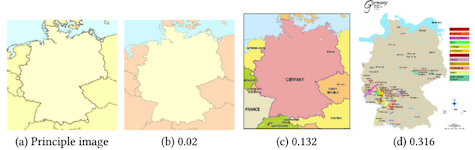
\includegraphics{master-thesis-preview}\\
& \href{https://drive.google.com/file/d/0B3Itc9NPxQ9VVWVUdUpGX19aVk0/view?resourcekey=0-D6vdMHOUJg1YMhIyrUIjAQ}{Refer to thesis report.}\\
\\
2014&{\bf Fieldwork to generate an Orthomosaic with aerial images acquired using a UAV.}\\
& 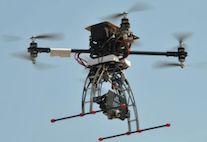
\includegraphics{orthomosaic-drone} 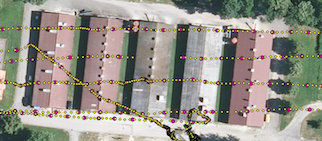
\includegraphics{orthomosaic-flightplan}\\ & \href{https://drive.google.com/file/d/1tSStjPzTilHk8CXQkhHDovqbnbbh6kTY/view?usp=sharing}{Refer to field report.}\\
\\
2014&{\bf Lab work to run a toy truck with a 3point controller around a predefined loop.}\\
& 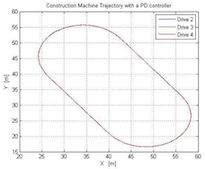
\includegraphics{self-driving-truck} \\ & \href{https://drive.google.com/file/d/191vUAqJYYORkw6q4UsV-o8fYL9f8-akC/view?usp=sharing}{Refer to lab report.}\\
\\
2011&{\bf Bachelor thesis on using Mathematical morphology for Rain gauge data for generating SKIZ maps and median maps.}\\
& 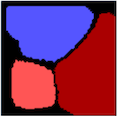
\includegraphics{weighted-skiz-map} \\ & \href{https://drive.google.com/file/d/1WU2PqMS-NAFZKoEmgEfDS05OKl5S7GVo/view?usp=sharing}{Refer to thesis report.}\\
\\
\end{tabular}
 
\end{document}